\section*{Net Neutrality}

\prob{4} Which of the following are commonly considered ``bright line'' rules
for Net Neutrality.\\ (Select all that apply.)\\
\correctanswercircle{No blocking} \\
\answercircle{No content moderation}\\
\correctanswercircle{No throttling}\\
\correctanswercircle{No paid prioritization}\\
\correctanswercircle{Transparency of practices}
\eprob


\prob{4} An Internet service provider notices a sudden uptick in streaming
video (e.g., Netflix, Amazon, etc.) traffic that is congesting certain network
links and interfering with other traffic, including latency-sensitive
applications such as gaming and video conference traffic.

To improve the performance of the network, the ISP decides to throttle
streaming video traffic so that the peak utilization never exceeds a couple of
megabits per second.  Would such throttling typically be considered a net
neutrality violation?
\yesnono
\eprob

\prob{4} Why or why not? \\
\answerbox{2.5}{ There is typically a carve-out for ``reasonable network
management'' in Net Neutrality rules.} \eprob

\pagebreak
\prob{4} Comcast and Netflix have, in the past, entered what is known as a
``paid peering'' agreement.  In such an agreement, Netflix pays Comcast to
connect directly to Comcast's network, rather than going through
intermediaries.  What are some reasons that Netflix would want to do this?\\
\correctanswercircle{Moving content closer to Comcast customers is likely to
improve streaming performance.}\\
\answercircle{Interconnecting with Comcast at an exchange point is completely free.}\\
\answercircle{Comcast would otherwise throttle Netflix traffic, unless it paid.}\\
\correctanswercircle{Directly connecting to Comcast saves the cost of transit through another ISP.}\\
\eprob


\prob{4} 
Explain why paid peering agreements are not typically considered a net
neutrality violation.
\answerbox{2}{}
\eprob

\section*{DNS Security and Privacy}

\prob{4} Which of the following are true about DNSSEC?\\
\correctanswercircle{DNSSEC provides integrity and authenticity for DNS records.}\\
\answercircle{DNSSEC provides confidentiality for DNS records.}\\
\correctanswercircle{DNSSEC uses public key cryptography.}\\
\answercircle{DNSSEC uses symmetric key cryptography.}\\
\eprob

\prob{4} Which of the following are true about DNS over HTTPS (DoH)?\\
\answercircle{DoH provides integrity and authenticity for DNS records.}\\
\correctanswercircle{DoH provides confidentiality for DNS records.}\\
\answercircle{DoH uses public key cryptography.}\\
\correctanswercircle{DoH uses symmetric key cryptography.}\\
\eprob

\prob{2} Is it possible to use both DNSSEC and DoH at the same time?\\
\yesnoyes
\eprob

\newpage
\section*{Web Privacy and Tracking}

Shown below is an image from the Lightbeam plugin, which we discussed in
class. It shows, for example, that {\tt fonts.gstatic.com} (a domain
maintained by Google) is a third-party
tracker that is contacted by many different websites.  

\begin{center}
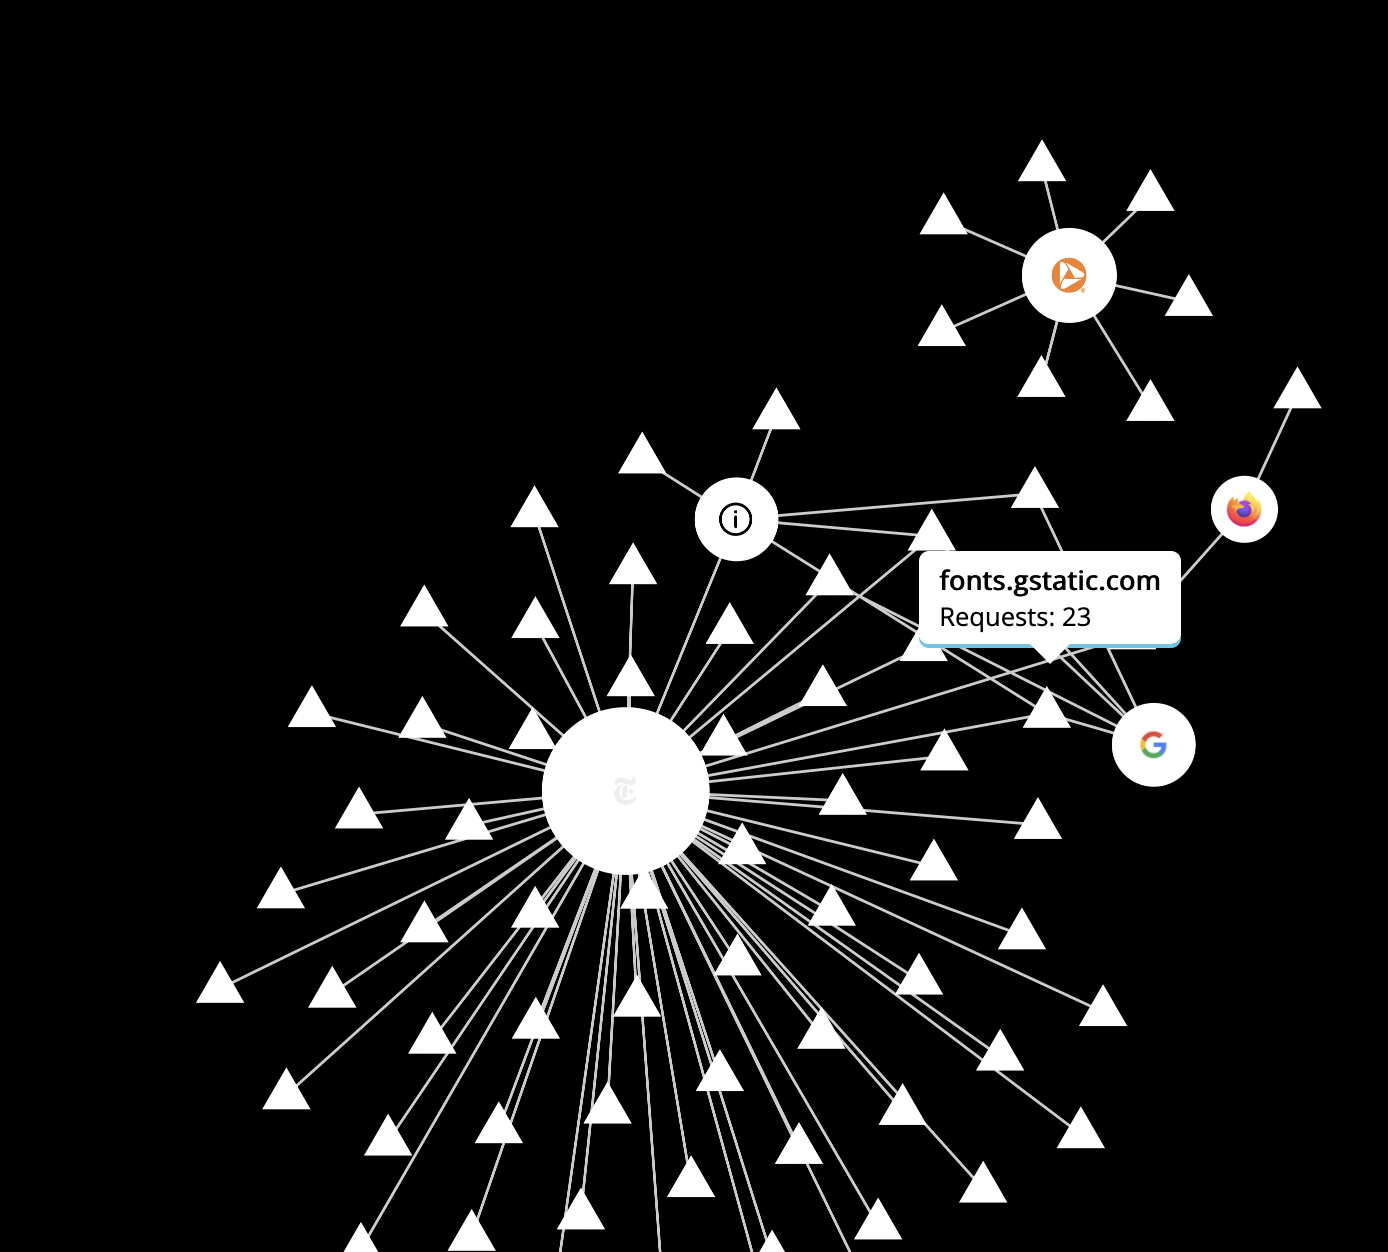
\includegraphics[width=0.5\textwidth]{lightbeam.png}
\end{center}

\prob{4} 
Why is it a potential problem that {\tt fonts.gstatic.com} is contacted by many
different websites?\\
\answerbox{2}{}
\eprob

\prob{4}
What types of information might Google be able to collect or infer about a user, given
the ability to track them across many different websites?\\
\correctanswercircle{Browsing history}\\
\correctanswercircle{Interests}\\
\answercircle{Credit card number}\\
\correctanswercircle{Name}\\
\eprob


\newpage
\section*{Vulnerability Disclosure}

\prob{2}
It is common practice to allow a company some period of time to fix a 
vulnerability before disclosing it publicly.  
\yesnono
\eprob

\prob{2}
Why or why not?\\
\answerbox{2}{}
\eprob

\if 0
\prob{4}
Responsible disclosure is a process by which a security researcher reports a
vulnerability to a vendor, and gives the vendor a chance to fix the
vulnerability before it is publicly disclosed.  What are some reasons that a
researcher might want to follow a responsible disclosure process?\\
\answerbox{2}{}
\fi

To improve security and catch vulnerabilities earlier, a company decides to
run a bug bounty program.  The company will pay \$1000 for each vulnerability
that is reported to them.  

\prob{4}
What are the potential benefits of such a program? \\
\answerbox{2}{}
\eprob


\prob{4}
What are the potential drawbacks? \\
\answerbox{2}{}
\eprob

\newpage
\section*{Digital Equity}

This topic was not covered as much in class, but there was an assignment on
it. So, there are not many points assigned to this section, and the questions
should be straightforward!

\prob{1}
Unreliable Internet access is only a problem in rural areas (i.e., not in cities).
\yesnono
\eprob

\prob{2}
A common metric to measure Internet performance is throughput, which is
measured in bits per second. What is a definition of throughput?  \\
\answerbox{2}{}
\eprob

\prob{4}
In the assignment, you worked with data from the FCC's Measuring Broadband
America program, which measures the performance of Internet service providers
(ISPs) in the United States.  What are some reasons that the FCC might want to
measure the performance of ISPs?\\
\correctanswercircle{To ensure that ISPs are providing the service that they
advertise.}\\
\answercircle{To ensure that ISPs are not providing service to customers in other countries.}\\
\correctanswercircle{To ensure that ISPs are providing service to customers in rural areas.}\\
\answercircle{To ensure that the service that ISPs are providing is affordable.}
\eprob

\pagebreak
\section*{Feedback}
\vspace*{-0.1in}
\prob{1}
Interest (1=Boring!; 10=Amazing!):
\shortanswerbox{0.5}{5}
Difficulty (1=Too easy; 10=Too hard):
\shortanswerbox{0.5}{5}
\eprob
\prob{1}
1. One topic you'd like to see covered that wasn't covered. 2. One other suggestion for
improvement.

\answerbox{0.75}{More free food.}
\eprob

